% This is LLNCS.DEM the demonstration file of
% the LaTeX macro package from Springer-Verlag
% for Lecture Notes in Computer Science,
% version 2.4 for LaTeX2e as of 16. April 2010
%
\documentclass{llncs}
\usepackage[font={small}]{caption, subfig}
\usepackage{microtype}
\usepackage{epsfig}
\usepackage{graphicx}
\usepackage{xcolor}
\usepackage{amsfonts,amsmath,amssymb}
\usepackage{fixltx2e} % Fixing numbering problem when using figure/table* 
\usepackage{subfig}
\usepackage{tabularx,ragged2e,booktabs}
\usepackage{float}
\DeclareMathSizes{10}{9}{6}{5}
\abovedisplayskip.50ex
\belowdisplayskip.50ex
\abovedisplayshortskip.50ex
\belowdisplayshortskip.50ex
%\restylefloat{figure}
%\restylefloat{table}
%\usepackage{todonotes}
%\usepackage{makeidx}  % allows for indexgeneration
%
\newcolumntype{C}[1]{>{\Centering}m{#1}}
\renewcommand\tabularxcolumn[1]{C{#1}}
\setlength{\parindent}{10pt}
\renewcommand{\tablename}{\bf Table}
%
%% Package to linebreak URLs in a sane manner.
\usepackage{url}
%% Define a new 'smallurl' style for the package that will use a smaller font.
\makeatletter
\def\url@smallurlstyle{%
  \@ifundefined{selectfont}{\def\UrlFont{\sf}}{\def\UrlFont{\small\ttfamily}}}
\makeatother
%% Now actually use the newly defined style.
\urlstyle{smallurl}
%% Define 'tinyurl' style for even smaller URLs (such as in tables)
\makeatletter
\def\url@tinyurlstyle{%
  \@ifundefined{selectfont}{\def\UrlFont{\sf}}{\def\UrlFont{\scriptsize\ttfamily}}}
\makeatother
\renewcommand{\UrlFont}{\scriptsize}
%
%% Make URLs clickable
\usepackage[colorlinks, bookmarks=false]{hyperref}
%\usepackage{hyperref}
\usepackage{breakurl}
\hypersetup{
    %linktoc=all,     %set to all if you want both sections and subsections linked
    %linkcolor=blue,  %choose some color if you want links to stand out
    colorlinks=false, %set true if you want colored links
    citecolor=black,
    filecolor=black,
    linkcolor=black,
    urlcolor=black
}
%\newcommand\abs[1]{\left|#1\right|}
%
\newcommand{\myfigureshrinker}{\vspace{-1cm}}
\newcommand{\bibfont}{\small}
\addtolength{\topmargin}{-9mm}
\addtolength{\topskip}{-6mm}
\addtolength{\textfloatsep}{-4mm}

\renewcommand\floatpagefraction{.9}
\renewcommand\topfraction{.9}
\renewcommand\bottomfraction{.9}
\renewcommand\textfraction{.1}   
\setcounter{totalnumber}{50}
\setcounter{topnumber}{50}
\setcounter{bottomnumber}{50}

\begin{document}
%
\mainmatter              % start of the contributions
%
\title{SAX-VSM: \\Time Series Classification Using SAX Representation and Vector Space Model}
%
\titlerunning{Timeseries features discovery with SAX and TF-IDF weighting}  
% abbreviated title (forrunning head)
%                                     also used for the TOC unless
%                                     \toctitle is used
%
\author{Pavel Senin\inst{1}
\and Sergey Malinchik\inst{2}
}
%
\authorrunning{Senin, P., Malinchik, S.} % abbreviated author list (for running head)
%
%%%% list of authors for the TOC (use if author list has to be modified)
%\tocauthor{Ivar Ekeland, Roger Temam, Jeffrey Dean, David Grove,
%Craig Chambers, Kim B. Bruce, and Elisa Bertino}
%
\institute{Collaborative Software Development Laboratory,\\
Information and Computer Sciences Department,\\
University of Hawaii at Manoa,\\ Honolulu HI 96822, USA,\\
\email{senin@hawaii.edu}
\and
Lockheed Martin Advanced Technology Laboratories,\\
3 Executive Campus, Suite 600, Cherry Hill, NJ 08002, USA,\\
\email{sergey.b.malinchik@lmco.com}}


\maketitle              % typeset the title of the contribution

\begin{abstract}
In this paper, we propose a novel method for characteristic patterns discovery in 
time series. This method, called SAX-VSM, is based on two existing techniques - 
Symbolic Aggregate approXimation and Vector Space Model. SAX-VSM is capable 
to automatically discover and rank time series patterns (features) by their 
“importance” to the class, which not only creates well-performing classifiers, 
but, in turn, provides interpretable class generalization and facilitates clustering. 
The accuracy of the method, as shown through experimental evaluation, is at the 
level of the current state of the art. 
While being relatively computationally expensive within a learning phase, 
our method provides fast, precise, and interpretable classification.
\keywords{Knowledge discovery, Algorithms, Experimentation}
\end{abstract}
%
\section{Introduction}
%
Time series classification is an increasingly popular area of the research. 
Within last decades, many time series representations, similarity measures, 
and classification algorithms were proposed \cite{review}. 
These, usually, can be divided in two major categories. 
The first category of classification techniques is based on the shape-based 
similarity metrics - where distance is measured directly between time series points. 
Examples of methods from this category are the classical nearest neighbor (kNN)
classifier built upon Euclidean distance \cite{1NN} and SpADe \cite{spade}. 
The second category consists of classification techniques based on the 
structural similarity metrics, which employ some high-level representations 
of time series. Examples from this category include DFT based classifier \cite{DFT}
and bag-of-patterns representation (BOP) \cite{bag_patterns}. 

The existence of these two categories can be explained by differences in the 
performance of these techniques. 
While shape-based similarity methods virtually unbeatable on short, 
often pre-processed, time series data \cite{benchmark}, 
they usually fail on long and noisy data sets \cite{indexing},
where feature-based techniques demonstrate a superior performance. 
Furtherer, feature-based methods require less storage space and, usually, 
have faster classification time, thus, they often implemented in industrial settings. 

As one of the possible alternatives to this two categories, recently, the time series shapelets
were introduced \cite{shapelet} and gained popularity. A shapelet is a \textit{short time 
series ``snippet''} that is a representative of class membership. Thus, potentially, this 
approach combines the best of two categories - the superior precision of shape-based 
similarity methods, and the high-throughput capacity and efficiency of feature-based 
methods.
%\cite{logical}. 
However, while demonstrating a superior interpretability, robustness, 
and similar to kNN algorithms performance, shapelets-based approaches are quite time-consuming 
- which makes their adoption for many-classes classification problems difficult \cite{bagnal}. 

As per current state of the art, it is worth noting, that despite to recent development, to date,
the best overall algorithm in the field is the simple nearest neighbor classifier, which is 
accurate and robust. Moreover, it depends on a very few parameters \cite{benchmark} 
\cite{comparison} \cite{classifiers}. Nevertheless, while possessing all these qualities,
1NN technique has a number of disadvantages, where the major is that it does not offer any 
insight into the data.

In this work, we propose yet another alternative to 1NN algorithm. Similarly to shapelets, our
technique rests on finding time series subsequences that are characteristic representatives of
classes. 
However, instead of iterative search for shapelets, our algorithm finds and weights by
``importance'' all potential candidate subsequences at once. 
In addition, being built upon SAX approximation which facilitates smoothing and elasticity, 
our technique performs well on noisy data.
All these, in turn, enable precise classification, clustering, and facilitate a discovery of 
characteristic patterns.

\section{Background}
Our methodology is based on two well-known techniques. The first technique is 
Symbolic Aggregate approXimation \cite{sax}, which is a high-level symbolic representation 
of time series data. The second technique is a well known in Information Retrieval (IR) 
Vector Space Model \cite{salton}. 
By utilizing SAX, our algorithm transforms labeled time series into collections of SAX 
words (terms). At the following step, it utilizes \textit{tf$\ast$idf} terms weighting for a 
classifier construction. The SAX-VSM classification relies on Cosine similarity metric.

SAX algorithm, however, requires three parameters to be provided as an input, and as per 
today, there is no efficient solution for parameters selection known to the best of our knowledge. 
To solve this problem, we employ a global optimization scheme that converges relatively quickly 
and yields a deterministic, optimized solution. 
This scheme is based on the divided rectangles (DIRECT) algorithm \cite{direct}, which is
a derivative-free global optimization process which does not require any parameters.
Furthermore, DIRECT possesses both local and global-optimization properties. 

\enlargethispage{0.5cm} 
\subsection{Symbolic Aggregate approXimation (SAX)}
Symbolic representation of time series, once introduced \cite{sax}, has attracted much attention by
enabling an application of numerous string-processing algorithms, bioinformatics, and text mining 
tools to temporal data. This method provides a significant reduction of the time series 
dimensionality and a low-bounding to Euclidean distance metric, which guarantees no false 
dismissal \cite{hot_sax}.
These properties are often leveraged by other techniques, which embed SAX representation in their
algorithms, notably shapelets, which \cite{fast-shapelets} utilize the dimensionality reduction and 
the low-bounding property for significant performance improvement.

Given a time-series $T$ of a length $n$, SAX produces its symbolic approximation $\hat{S}$ of 
a length $w$ where letters are taken from an alphabet $\alpha$. 
Along with $T$, two parameters must be specified as the input: an alphabet size $\alpha$ and 
a size of the word to produce $w$. Algorithm works as follows. 

First of all, since SAX rests on the assumption that normalized time series tend to have Gaussian 
distribution \cite{larsen_marx}, the time-series $T$ is normalized. 
At the second step, the dimensionality of the normalized time series is reduced to $w$ by 
obtaining a Piecewise Aggregate Approximation (PAA) of $T$. 
Specifically, this approximation is obtained by dividing the time series $T$ into $w$ 
equal-sized segments and computing the mean values for points within each segment. 
The aggregated sequence of these mean values forms PAA approximation of $T$ of length $w$.
Finally, each of PAA coefficients is converted into a letter of the alphabet $\alpha$ by the use 
of lookup tables. These tables are built by defining a set of breakpoints that divide the 
distribution space into $\alpha$ equiprobable regions \cite{sax}.

\subsection{Bag of words representation of time series} \label{bow_representation}
Following its introduction, SAX was shown to be an efficient tool for solving problems 
of finding motifs and discords in time series \cite{motifs} \cite{hot_sax}. 
The authors employed a sliding window based subsequence extraction technique 
and augmented data structures (hash table in \cite{motifs} and trie in \cite{hot_sax}) 
in order to build SAX words ``vocabularies''. Further, by analyzing words frequencies 
and locations, they were able to capture frequent and rare SAX words representing 
motifs and discords subsequences. Later, the same technique based on the combination 
of sliding window and SAX was used in the numerous works, most notably in time series 
classification using bag of patterns \cite{bag_patterns}. 

We use this sliding window technique to convert a time series $T$ of a length $n$ into 
the set of $m$ SAX words, where $m=(n-l_{s})+1$ and $l_{s}$ is the sliding window length. 
By sliding a window of length $l_{s}$ across time series $T$, extracting subsequences, 
converting them to SAX words, and placing these words into an unordered collection, 
we obtain the \textit{bag of words} representation of the original time series $T$.

\subsection{Vector Space Model (VSM)}
We use Vector space model exactly as it is known in information retrieval (IR) - 
for disambiguating class entities \cite{salton}. Similarly to IR, we define and use 
terms \textit{document}, \textit{bag of words}, \textit{corpus}, and 
\textit{sparse matrix} in our workflow. 
Note however, that terms \textit{bag of words} and \textit{document} are used 
interchangeably for abbreviation of an unordered collection of SAX words, while 
in IR these usually bear different meaning, where a \textit{document} usually 
presumes certain words ordering (semantics). 
Although, similar definitions, such as \textit{bag of features} or 
\textit{bag of patterns}, were previously proposed for techniques built upon 
SAX \cite{bag_patterns}, we use \textit{bag of words} since it reflects our 
workflow precisely. The term \textit{corpus} is used for a structured collection 
of bags of words. 

Given a training set, SAX-VSM builds bags of SAX-generated words representing 
each of the training classes and assembles them into a corpus. 
This corpus, by its construction, is a sparse \textit{term frequency matrix}. 
Rows of this matrix correspond to the set of all SAX words found in 
\textit{all classes}, while each column of the matrix denotes a class of the 
training set. Each element of this matrix is an observed frequency of a word
in a class. 
Many elements of this matrix are zeros - because words extracted from one class 
are often not found in others 
%(Figure \ref{fig:venn}). 
By its design, this sparse 
term frequency matrix is a dictionary of all SAX words extracted from all time 
series of a training set, which accounts for frequencies of each word in each of 
the training classes.

Following to the common in IR workflow, we employ the \textit{tf$\ast$idf} weighting 
scheme for each element of this matrix in order to transform a frequency value into
the weight coefficient. 
The \textit{tf$\ast$idf} weight for a term is defined as a 
product of two factors: term frequency (\textit{tf}) and inverse document 
frequency (\textit{idf}). 
For the first factor we use logarithmically scaled term frequency:
\begin{equation}
 \mbox{tf}_{t, d} =  \begin{cases} \log(1 + \mbox{f}_{t,d}), &\mbox{if f}_{t,d}>0  \\
0, & \mbox{otherwise} \end{cases}
\end{equation} 
where $t$ is the term, $d$ is a bag of words (a \textbf{d}ocument), and $\mbox{f}_{t,d}$ 
is a frequency of the term in a bag.

The inverse document frequency we compute as usual:
\begin{equation}
 \mbox{idf}_{t, D} =  \log_{10}\frac{|D|}{|d \in D : t \in d|} = \log_{10}\frac{N}{\mbox{df}_{t}}
\end{equation} 
where $N$ is the cardinality of corpus $D$ (the total number of classes) and the 
denominator $\mbox{df}_{t}$ is a number of documents where the term $t$ appears.

Then, $\textit{tf$\ast$idf}$ value for a term $t$ in the document $d$ of a corpus $D$ is defined as 
\begin{equation}
 \mbox{tf * idf}(t, d, D) =  \mbox{tf}_{t, d} \times \mbox{idf}_{t, D} = \log(1 + \mbox{f}_{t,d})
\times \log_{10}\frac{N}{\mbox{df}_{t}}
 \label{formula:tfidf}
\end{equation} 
for the all cases where $\mbox{f}_{t,d}>0$ and $\mbox{df}_{t}>0$, or zero otherwise.
Once all terms of a corpus are weighted, the columns of a sparse matrix are used 
as class \textit{term-weight vectors} which facilitate the classification using Cosine similarity. 

Cosine similarity measure between two vectors is based on their inner product. 
For two vectors $\boldsymbol{a}$ and $\boldsymbol{b}$ that is:
\begin{equation}
%\mbox{similarity}(\boldsymbol{a},\boldsymbol{b}) = cos(\theta) = \frac{ \sum\limits^{n}_{i=1} a_{i}
%\times b_{i} }{
%\sqrt{\sum\limits^{n}_{i=1} a_{i}} \times \sqrt{\sum\limits^{n}_{i=1} b_{i}} }
\mbox{similarity}(\boldsymbol{a},\boldsymbol{b}) = cos(\theta) = \frac{ 
\mathbf{a} \mathbf{b} } {\left| \left| a \right| \right| \left| \left| b \right| \right|}
\end{equation} 

\subsection{A note on numerosity reduction}
In further SAX development, particularly in its application for discords discovery,
streaming data analyses, and clustering \cite{hot_sax} \cite{streaming_sax}, the authors 
proposed a combination of a sampling strategy and a distance function specifically 
designed in order to avoid ``trivial and degenerative solutions''. While the inclusion of
numerosity reduction was found to be vital for mentioned SAX applications, intuitively, 
in our case, the over-counting effect is significantly mediated by \textit{tf$\ast$idf}
statistics \eqref{formula:tfidf}. Moreover, by enforcing the exclusion of ``trivial matches'', we
may degrade the overall classification accuracy of SAX-VSM, as pointed in 
BOP work \cite{bag_patterns}.

To clarify this issue, we experimented with original combination of a sampling strategy 
and a distance function and found it useful in the parameters optimization scheme. 
For most of the datasets, inclusion of the reduction significantly reduced the DIRECT 
scheme convergence time and improved its accuracy. 
Moreover, once we relaxed the ``triviality constraints'' by substitution of 
\textit{MINDIST} function \cite{streaming_sax} with Hamming distance \cite{hamming}, 
we were able to improve the SAX-VSM classification accuracy for fourteen 
out of thirty one datasets we used for validation (see \cite{jmotif}).
%
%Thus, we shall explain this in greater detail.
%As noted in \cite{sax}, given a character subsequence $\hat{S_{i}}$ extracted by the use 
%of sliding window and SAX, it is very likely, that $\hat{S_{i}}$ is very similar to its
%neighboring subsequences, $\hat{S_{i-1}}$ and $\hat{S_{i+1}}$ (i.e. those that start one 
%point to the left, and one point to the right of $\hat{S_{i}}$), especially if $\hat{S_{i}}$
%is in the smooth region of the time series - due to the dimensionality reduction. 
%This phenomena results in mapping of multiple consecutive subsequences
%to the same string. The authors called these subsequences as ``trivial matches'' of 
%$\hat{S_{i}}$, and suggested to avoid their over-counting by introducing a 
%``numerosity reduction technique''. This technique is based on the custom distance 
%function \textit{MINDIST} \cite{streaming_sax}, and accounts only for the first 
%occurrence of $\hat{S_{i}}$. 
%
%Similarly to \textit{MINDIST} we define a $dist$ function for two
%SAX words $\hat{Q}$ and $\hat{C}$ as
%\begin{equation}
 %dist(\hat{q_{i}},\hat{c_{i}})=
        %\begin{cases} \qquad  0, & \mbox{, if } | \hat{q_{i}} - \hat{c_{i}} | \leq 1 \\
         %ASCIIdist( \hat{q_{i}} , \hat{c_{i}} ) & \mbox{, otherwise } 
        %\end{cases}
%\end{equation} 
%where $ASCIIdist( \hat{q_{i}}, \hat{c_{i}} )$ is the absolute value of the difference between 
%ASCII codes for letters $\hat{q_{i}}$ and $\hat{c_{i}}$.
%
%By using this function we modified the process a bag of words construction: 
%while sliding a window across a time series and extracting consecutive words
%as explained in Section \ref{bow_representation}, we compare each newly 
%extracted word to the last word added to the bag using $dist$ function. 
%If these words appear to be equal, we discard the new (to be added) word and 
%continue as usual. Since this numerosity reduction strategy is based 
%on previous work we called it $CLASSIC$.
%
%By further experimentation, we discovered, that if we relax this numerosity reduction
%strategy by using Hamming distance \cite{hamming} instead of $dist$ function
%defined above, it is possible to further improve SAX-VSM accuracy for fourteen 
%out of thirty one datasets we used for validation (see \cite{jmotif}). 
%We called this numerosity reduction strategy EXACT, since the use of Hamming 
%distance prevents only exact consecutive trivial matches to be placed into the bag. 

At this point we unable to further comment on these experimental results and 
leaving this phenomena for the future research.

\section{SAX-VSM classification algorithm }
As many other classification techniques, SAX-VSM consists of two parts - the training phase 
and the classification. In the following sections we shall explain the algorithm in greater detail 
while this section presents its overview and its main differences from other techniques.

The training phase of the SAX-VSM classifier is relatively computationally expensive 
(Fig. \ref{fig:precision-runtime}) because it involves construction of a corpus by
extraction of SAX words from all labeled series and its post-processing with VSM. 
However, there is no need to maintain an index of training series, or to keep any of 
them in the memory at runtime: the algorithm simply iterates over all labeled series
incrementally building bags of SAX words for each of the training classes, 
that is, algorithm builds a \textit{single bag of words for each training class}. 
Once built, the corpus of $N$ bags of words (where $N$ is the number of classes) is
processed with \textit{tf$\ast$idf} and can be also discarded. 
Only the set of $N$ real-valued vectors is retained after training for classification. 
Note, that the construction of a single bag for each of training classes is a one 
of the main differences of SAX-VSM from other previously published 
techniques \cite{bag_patterns}.

The classification phase of the SAX-VSM is fast and consists of converting of an 
unlabeled time series into a bag of words and its successive classification by 
computation of $N$ cosine values. The unlabeled time-series is then assigned to 
the class with which the cosine similarity is maximal. The use of the cosine 
similarity is another main difference of SAX-VSM from competing techniques.

\begin{figure}[t]
   \centering
   \myfigureshrinker
   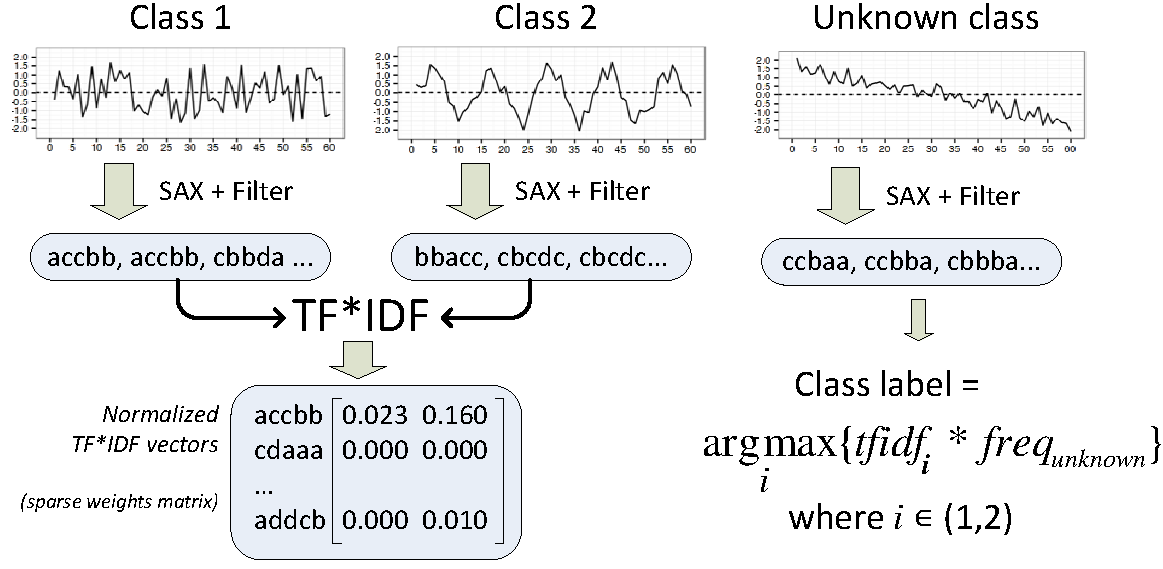
\includegraphics[width=115mm]{figures/overview.eps}
   \caption{
   An overview of the SAX-VSM algorithm: 
   at first, labeled series are converted into bags of words using SAX; 
   secondly, \textit{tf$\ast$idf} statistics is computed resulting in 
   a single weights vector per training class. An unlabeled series is converted 
   into the bag of words, and assigned the label of a weight vector with which 
   the angle is minimal (i.e. the cosine similarity is maximal).}
   \label{fig:overview}
\end{figure}

\subsection{Training phase}
In order to use Vector Space Model, we need to transform all labeled time-series into 
symbolic representation.  For this, our algorithm converts a real valued time series 
into SAX string representation configured by four parameters: the sliding window
length (\textit{W}), the number of PAA frames per window (\textit{P}), the SAX alphabet size
(\textit{A}), and by the numerosity (complexity) reduction strategy (\textit{S}). 
As we mentioned, each of the extracted with sliding window subseries is z-normalized
before being processed with PAA.
%\cite{goldin_kanellakis}. 
If, however, 
the standard deviation of the time-series values is below a fixed epsilon threshold, 
we do not apply this normalization.

By applying this procedure to all $N$ training classes, we build a corpus of $N$ bags, 
which, in turn, we process with \textit{tf$\ast$idf}. This provides $N$ real-valued 
vectors of equal length representing training classes. 

\subsection{Classification phase}
Similarly to training phase, in order to classify an unlabeled time-series, we transform it into the
terms vector using the same sliding window technique and SAX parameters which were used 
in the training phase. Then, we compute Cosine similarities between this terms vector and 
\textit{tf$\ast$idf} weight vectors representing $N$ labeled classes. 
The series is assigned to the class whose vector yields the maximal Cosine similarity value.

\begin{figure}[t]
   \myfigureshrinker
   \centering
   \includegraphics[width=115mm]{figures/figure_direct.eps}
   \caption{Illustration of parameters optimization with DIRECT 
   for \textit{SyntheticControl} dataset. 
   Left panel shows all points sampled by DIRECT in the space $PAA*Window*Alphabet$; here
   red points correspond to high error values in cross-validation experiments, while green color 
   indicates low error values. Note the green points concentration at $W$=42.\\ 
   Middle panel shows the error-rate heat map when the sliding window size is fixed to 42, 
   this figure was obtained by a complete scan of all 432 points of the slice.\\ 
   Right panel shows the optimized by DIRECT sampling. The optimal solution 
   ($W$=42,$P$=8,$A$=4) was found by sampling of 43 points.}
   \label{fig:direct-sampling}
\end{figure}

\subsection{SAX parameters selection} \label{section-direct}
We use a common cross-validation scheme while exploring possible parameters space. 
In order to accelerate the search for optimal set, 
we utilize DIRECT (DIviding RECTangles) algorithm, which 
was introduced by Jones et al. \cite{direct-original}. This optimization scheme 
designed to search for global minima of a real valued function over a bound-constrained domain. 
In our implementation we use rounding of parameters by nearest integer function.

The algorithm iteratively performs two procedures - partitioning the search domain, 
and identifying potentially optimal hyper-rectangles (i.e., having potential to contain good
solutions). 
It begins by scaling the search domain to a n-dimensional unit hypercube which is considered 
as potentially optimal. The error function is then evaluated at the center of this hypercube. Next, 
other points are created at one-third of the distance from the center in all coordinate directions. 
The hypercube is then divided into smaller rectangles which are identified by their center point 
and their error function value. This procedure continues interactively until error function
converges.
For brevity, we omit the detailed explanation of the algorithm, and refer the 
interested reader to \cite{direct} for additional details about our implementation.

\subsection{Intuition behind SAX-VSM}
First of all, by combining \textit{\textbf{all}} SAX words observed in \textit{\textbf{all}}
time series of single class into a single bag of words, SAX-VSM manages to exhaustively 
capture intraclass variability similarly to 1NN classifiers.  

Secondly, by partially discarding the original ordering of time series subsequences, and
through subsequence normalization, SAX-VSM is capable to capture characteristic 
subsequences in compressed and stretched time series, as well as to recover a signal 
from noisy and corrupted data. 

Thirdly, the \textit{tf$\ast$idf} statistics naturally ``highlights'' the terms unique to the
class by assigning them higher weights, while terms observed in a number of classes are 
assigned weights inversely proportional to their interclass presence frequency. 
This weighting scheme naturally improves the selectivity of classification 
by  lowering the contribution of ``confusive'' multi-class terms, and  increasing  the 
contribution  of  class' ``defining'' terms to the final similarity value.   

When combined, these particular specificities make SAX-VSM time series classification 
approach unique: basically, within a classification phase, it compares a set of short 
overlapping subsequences extracted from a full length of an unlabeled time series with 
sets of weighted characteristic subsequences representing training classes.
Thus, an unlabeled time series is assigned a label by its similarity not to a fixed number 
of sequences (as in kNN classifiers) or to a fixed number of features (as in shapelet-based 
classifiers) but by a value of product of its subsequences similarity to all known subsequences.
This, as we shall show, contributes to the excellent classification performance on temporal 
data sets where time series have very low intraclass similarity at the full length, but 
embed characteristic for classes subsequences. In particular, note SAX-VSM performance 
on Electrical Devices data set \ref{perf_table}, and our previous experimental results on 
software process artifact trails \ref{trajectory}.
   
\section{Results}
We have proposed a novel algorithm for time series classification based on the SAX
representation of time series and Vector space model called SAX-VSM. Here, we present a range of
experiments assessing its performance in classification and clustering.

\begin{small}
\begin{table}[t]
\caption{\bf Classifiers error rates comparison.}
 \label{perf_table}
\centering
\begin{tabularx}{\linewidth}{@{} l *5X @{}}\toprule[1.5pt]
\bf Dataset &\bf 1NN-Euclidean &\bf 1NN-DTW &\bf Shapelet Tree &\bf  Shapelet SVM &\bf 
SAX-VSM\\\midrule
%\bf Variable Name & \bf Regression 1 & \bf Mean & \bf Std. Dev & \bf Min & \bf Max\\\midrule
%text        &  text     & text      &  text     &  text     &text\\
%\bottomrule[1.25pt]
%\end {tabularx}
%\begin{tabular}[h]{  l | c | c | c | c |  c  }
%\hline
%Dataset           & 1NN-Euclidean  & 1NN-DTW       & Shapelet Tree & Shapelet SVM & SAX-VSM \\
%\hline
SyntheticControl  & 0.120   & \textbf{0.007}  & 0.057     & 0.127            & 0.010 \\
Adiac             & 0.389   & 0.396           & 0.700        & 0.762         & \textbf{0.381}\\
Beef              & 0.467   & 0.467           & 0.500        & 0.133         & \textbf{0.033}\\
ChlorineConcentration  & 0.350 & 0.350        & 0.412        & 0.439         & \textbf{0.332} \\
Coffee            & 0.250   & 0.180           & 0.036     & \textbf{0.0}     & \textbf{0.0} \\
ECG               & 0.120   & 0.230           & 0.149     & \textbf{0.007}   & 0.09 \\
ElectricDevices   & 0.913   & 0.913           & 0.451     & 0.756            & \textbf{0.329} \\
FaceFour          & 0.216   & 0.170           & 0.159     & 0.023            & \textbf{0.0} \\
Gun Point         & 0.087   & 0.093           & 0.107     & \textbf{0.0}     & 0.007 \\
Lightning7        & 0.425   & \textbf{0.274}  & 0.507     & 0.314            & 0.301 \\
SonyAIBO          & 0.306   & 0.274           & 0.155     & \textbf{0.133}   & 0.176 \\
Trace             & 0.240   & \textbf{0.0}    & 0.020     & 0.020            & \textbf{0.0} \\
\bottomrule[1.25pt]
\end{tabularx}
\end{table}
%\hline
%\end{tabular}
\end{small}

\subsection{Analysis of classification accuracy}
To evaluate our approach, we selected thirty one data set. Majority of the data sets was taken 
from the UCR time series repository \cite{ucr}, the Ford data was originally used in a competition
at the IEEE World Congress on Computational Intelligence \cite{ford}, the Electrical Devices
dataset was downloaded from supporting website for \cite{bagnal}. Overall, SAX-VSM classification 
performance found to be at the level of best performing 1-NN classifiers (whether based on 
Euclidean distance, DTW, or SAX), shapelet tree, or a shapelet-based SVM. 
This result is not surprising taking in account ``No Free Lunch theorems'' \cite{nfl}, which 
assert, that there will not be a single dominant classifier for all TSC problems.

Table \ref{perf_table} compares the performance of SAX-VSM and four competing classifiers: 
two 1NN classifiers based on Euclidean distance and DTW, and two classifiers 
based on the recently proposed shapelet technique: the shapelet decision tree \cite{shapelet}
%\cite{logical} 
classifier and the shapelet transform classifier \cite{bagnal}. We use these 
particular datasets, because they represent a subset for which we were able to collect
classification accuracy results of all four classifiers. 
The performance of SAX-VSM for the rest of data sets can be found online along with 
our reference implementation \cite{jmotif}.

In our evaluation we followed train/test split of the data. We exclusively used train data in 
cross-validation experiments for selection of SAX parameters and numerosity reduction strategy
using DIRECT (Section \ref{section-direct}). Once selected, the optimal set of parameters 
was used to assess SAX-VSM classification accuracy which is reported in the last column 
of the Table \ref{perf_table}.


\begin{figure}[t]
   \myfigureshrinker
   \centering
   \includegraphics[width=115mm]{figures/precision-runtime.ps}
   \caption{Comparison of classification precision and runtime of SAX-VSM and 1NN 
   Euclidean classifier on CBF data. SAX-VSM performs significantly better with limited 
   amount of training samples (left panel). While SAX-VSM is faster in time series 
   classification, its performance is comparable to 1NN Euclidean classifier when 
   training time is accounted for (right panel).}
   \label{fig:precision-runtime}
\end{figure}

\enlargethispage{0.5cm} 
\subsection{Scalability analysis}
For synthetic data sets, it is possible to create as many instances as one need for experimentation.
We used CBF data set \cite{cbf} to investigate the performance of SAX-VSM and 1NN Euclidean
classifier on increasingly large training data sets of size 10, 50, 125, ..., 1000, and a fixed test
dataset of 10000 instances. For small training data sets, SAX-VSM is significantly more accurate
than 1NN Euclidean classifier, however, by the time we had more than 500 time series in
our training set, there was no statistically signifiant difference in accuracy (Fig.
\ref{fig:precision-runtime}). 
As per classification runtime cost, SAX-VSM was found more expensive than 1NN Euclidean classifier
when training set is small mostly due to the training cost. For the large training sets, there was
no significant difference in the overall runtime speed for both classifiers.
However, SAX-VSM allows to perform training offline and load \textit{tf$\ast$idf} weights vector as
needed. If this option utilized, the classification time cost is always significantly less than that
of 1NN Euclidean classifier (Fig. \ref{fig:precision-runtime}).

\subsection{Robustness to noise}
In our experimentation we observed, that the dimension of \textit{tf$\ast$idf} weights vectors 
grows following the grows of the training set size. 
%While it grows rapidly at the beginning, once
%the dictionary is saturated, growth tend to slow down (left panel of Figure \ref{fig:corrupted}). 
%Nevertheless, by adjusting alphabet and PAA sizes it is possible to keep the number of terms
%significantly large. 

%\begin{figure}[t]
%   \centering
%   \includegraphics[width=120mm]{figures/Venn.eps}
%   \caption{Left panel: illustration of terms growth for CBF corpus and individual classes with 
%   training set size. Right panel: distribution of SAX terms in CBF corpus for training set of 
%   1000 series of each class.}
%   \label{fig:venn}
%\end{figure}
This observation, and the fact that each of SAX words is covering only a small part of time 
series, prompted the idea that SAX-VSM classifier might be robust to the loss of signal 
in unlabeled series. Intuitively, in such a case, the cosine similarity might not
degrade significantly enough to cause misclassification.

While we plan to perform more exploration, current experimentation with CBF dataset revealed 
promising results. In one series of experiments, we randomly replaced up to fifty percent of a
time series span with a random noise and found, that SAX-VSM is performing consistently better 
than 1NN Euclidean classifier regardless of a training set size which we varied from five to
ten thousands (Fig.\ref{fig:corrupted}). 
In another series of experiments, we introduced a random noise into unlabeled
series, ranging its varying its standard deviation up to XX percent. In this experiments, SAX-VSM
also performed significantly better than 1NN Euclidean classifier (Fig.\ref{fig:corrupted}). 
However, this result we attribute to the PAA and SAX ability to withstand the noise.

\begin{figure}[t]
  \myfigureshrinker
  \centering
  
\includegraphics[width=115mm]{figures/corrupted.ps}
  \caption{Left panel: Illustration of classification performance with presence of noise
 (left panel),  and with signal loss (right panel).}
  \label{fig:corrupted}
\end{figure}

\subsection{Exploratory data analysis}
While classification results reported in previous section show that SAX-VSM classifier
has very good potential, one of the strengths of using it as a classification tool is that
it facilitates a superior level of interpretation when compared with other techniques. 

Previously, in original shapelets work \cite{shapelet}, it was shown 
that the resulting decision trees provide interpretable classification and an insight into the data
specific features. In successive work \cite{bagnal} based on shapelets, it was shown that
discovery of multiple shapelets provides even better intuition into interpretability of
classification. However, the authors noted, that a time cost of multiple shapelets discovery
could be significant. Contrary, SAX-VSM provides numerous weighted patterns at no time cost
allowing further insight into interpretability.

\begin{figure}[t]
   \myfigureshrinker
   \centering
   \includegraphics[width=115mm]{figures/gun-point.eps}
   \caption{Examples of best weighted patterns from each class of \textit{GunPoint} dataset. 
   Note, that while the upward arm motion is more ``important'' for a \textit{Gun} class, 
   the downward arm motion better characterizes \textit{Point} class. 
   This result aligns with previous work \cite{shapelet} and \cite{bagnal} in which similar 
   locations for best discriminative patterns were reported. 
   Second to the best patterns outline differences between aiming in \textit{Gun} class and
   smooth, propless hand movement in \textit{Point} class.
   }
   \label{fig:shapelet-like-patterns}
\end{figure}

\subsection{Gun Point data}
Following previously mentioned shapelet-based work \cite{shapelet} and\cite{bagnal}, 
we used a well-studied \textit{GunPoint} data set \cite{gun} to explore the 
interpretability of classification results. This data set contains two classes: 
time-series in \textit{Gun} class correspond to the actors hands motion when drawing a 
a replicate gun from a hip-mounted holster, pointing it at a target for a second,
and returning the gun to the holster; 
time-series in \textit{Point} class correspond to the actors hands motion when pretending
of drawing a gun - the actors point their index fingers to a target for about a second, 
and then return their hands to their sides. 

Similarly to previously reported results \cite{shapelet} \cite{bagnal}, 
SAX-VSM was able to capture all distinguishing features as shown at the 
Figure \ref{fig:shapelet-like-patterns}. The most weighted by SAX-VSM patterns in 
\textit{Gun} class corresponds to fine extra movements required to lift and aim the prop. 
The most weighted SAX pattern in \textit{Point} class corresponds to the ``overshoot''
phenomena which is causing the dip in the time series. 
Also, similarly to the original work \cite{gun}, SAX-VSM highlighted as second to the best
patterns in \textit{Point} class the lack of distinguishing subtle extra movements required
for lifting a hand above a holster and reaching down for the gun.

\begin{figure}[t]
   \myfigureshrinker
   \centering
   \includegraphics[width=115mm]{figures/AcerCircunatum.eps}
   \caption{Illustration of the best discriminating patterns found by SAX-VSM for
\textit{OSULeaf dataset}. These patterns align with well known in botany discrimination techniques
by lobe shapes, serrations, and the leaf tip type.}
   \label{fig:shapelet-acer-patterns}
\end{figure}

\subsection{OSU Leaf data}
According to the original data source, Ashid Grandhi \cite{osuleaf}, with the current growth of
digitized data, there is a huge demand for automatic management and retrieval of various images. The
\textit{OSULeaf} dataset consist of curves obtained by color image segmentation and boundary
extraction (in the anti-clockwise direction) from digitized leaf images of six classes: \textit{Acer
Circinatum, Acer Glabrum, Acer Macrophyllum, Acer Negundo, Quercus Garryana and Quercus Kelloggii}.
While the authors of the original work were able to solve the problem of leaf boundary curves
classification by use of DTW achieving 60\% accuracy, DTW, as we pointed above, provides a very
little information about why it succeeds of fails. 

In contrast, SAX-VSM application yielded a set of class-specific characteristic patterns for each of
six leafs classes from the \textit{OSULeaf} dataset which closely match known techniques of leafs
classification based on leaf shape and margin \cite{dirr}. These features include the slightly
lobed shape and acute tips of Acer Circinatum leafs, serrated blade of Acer Glabrum leafs,
the accuminate tip and characteristic serration of in Acer Macrophyllum leafs, pinnately compound
leafs arrangement of Acer Negundo, the incised leaf margin of Quercus Kelloggii, and a lobed leaf
structure of Quercus Garryana. Figure \ref{fig:shapelet-acer-patterns} shows three of these classes
along with their highlighted features at leafs images and within corresponding class time series.

Further, we found, that in the \textit{Coffee} spectrogram dataset SAX-VSM highlighted spectrogram
intervals corresponding to Caffeine and Chlorogenic acid - two chemical compounds responsible for
the differences in coffee flavor, which also aligns with previously reported findings \cite{coffee}.
\section{Clustering}
Clustering is a common tool used for data partitioning, visualization and exploration. Furthermore, 
clustering serves as an important subroutine in many other data mining algorithms.
\begin{figure}[t]
   \myfigureshrinker
   \centering
   \includegraphics[width=115mm]{figures/clustering.eps}
   \caption{A comparison of hierarchical clustering application to a subset 
\textit{SyntheticControl} classes: \textit{Normal, Decreasing trend}, and \textit{Upward shift}. 
Euclidean distance, Dynamic time warping, SAX-VSM and Complete linkage were used to 
generate these plots. Only SAX-VSM was able to partition series properly.                           
   }
   \label{fig:hc}
\end{figure}

\subsection{Hierarchical clustering}
Probably, one of the most used clustering algorithms is hierarchical clustering which requires no
parameters to be specified \cite{hcs}. It computes pairwise distances between all objects and 
produces a nested hierarchy of the clusters offering a great data visualization power. 

Previously, it was shown that the bag-of-patterns representation of time-series
provides is superior clustering performance when Euclidean distance is used \cite{bag_patterns}. 
We performed similar experiments which differ in time series representation and distance
metrics - we relied on \textit{tf$\ast$idf} weights vector and Cosine similarity. 
Affirming the previous work, we found, that the combination of SAX and Vector space model
outperforms other distance metrics. For example, figure \ref{fig:hc} depicts the result 
of hierarchical clustering of a subset of \textit{SyntheticControl} data set which
includes \textit{normal, decreasing trend}, and \textit{upward shift} time series.
As one can see, SAX-VSM is superior in clustering performance to Euclidean and DTW distance 
metrics in this particular setup, producing a hierarchy, which properly partitions the data set 
into three branches.

\subsection{k-Means clustering} \label{trajectory}
Another popular choice for data partitioning is a k-Means clustering algorithm \cite{kmeans}.
The basic intuition behind this algorithm is that through the iterative reassignment of objects 
into different clusters the intra-cluster distance is minimized. As was shown, kMeans 
algorithm scales much better than hierarchical partitioning techniques \cite{kscale}.
Fortunately, this clustering technique is well studied in IR field. Previously, in \cite{zhao}, the
authors extensively examined seven different criterion functions for partitional document
clustering and found that \textit{k}-prototypes partitioning with cosine dissimilarity delivers a
very good performance. 

We implemented a similar to \cite{modha} \textit{spherical k-means algorithm} and found through
experimentation, that algorithm converges quickly delivering satisfactory partitioning on
short, synthetic datasets. In addition, we evaluated our technique on the long time series 
originating from PhysioNet archive \cite{physionet}. We extracted 250 series corresponding
to five vital signals: two ECG leads, RESP wave, PLETH wave, and  CO2 wave,
trimming them to 2'048 points. Similarly to \cite{bag_patterns}, we run a reference k-Means 
algorithm implementation based on Euclidean distance, which achieved the maximum 
clustering quality of 0.39, when measured as proposed in \cite{kmetrics} on the best 
clustering (the one with the smallest objective function in 10 runs). 
SAX-VSM k-Means implementation outperformed the reference technique yielding clusters 
with a quality of 0.67 (for a $W$=33, $P$=8, $A$=6).

Note also, that previously, we applied our implementation to recurrent behaviors (motifs) 
discovery in software development telemetry streams\cite{android}. 
These behavioral time series were extracted from software change repositories and are 
structurally similar to \textit{ElectricDevices} dataset. 
We have used the bag of words time series representation and spherical k-Means clustering 
in order to discover specific temporal features corresponding to the software release cycle. 
Specifically, we optimized SAX parameters in order to obtain a proper partitioning of known 
development behaviors before and after the software release. In turn, the centroids of these 
clusters represented by \textit{tf$\ast$idf} weights vectors were used to classify unlabeled  
temporal intervals. This technique allowed us to successfully classify pre- and post-release
behaviors with accuracy above eighty percents.

\section{Conclusion and Future Work}
In this paper, we have proposed a novel technique for time series classification based on 
characteristic patterns discovery. We have shown, that our approach is competitive with, 
or superior to, other techniques on a variety of classic data mining problems. In addition, 
we described several advantages of SAX-VSM over existing structure-based similarity measures.
Specifically, it is capable to simultaneously consider local and global structural similarity by 
using short overlapping time series subsequences and Vector space model. 
In addition, by employing \textit{tf$\ast$idf} weighting scheme, SAX-VSM allows users to 
discriminate time series subsequences by their class characterization power.

The current limitations of our SAX-VSM implementation suggest a number of future work directions. 
First of all, while Vector space model naturally supports processing of bags of words composed 
of terms of variable length, our implementation lacks this capacity. We prioritize the development in 
this direction inspired by the recently reported superior performance of multi-shapelets based
classifiers \cite{bagnal}.
Secondly, the choice of optimal parameter set for SAX-VSM remains challenging.
While DIRECT optimization provides satisfiable performance, it is designed for a function of a real 
variable. By using rounding in our implementation, we have observed DIRECT iteratively sampling 
redundant locations. 
Finally, we are working on the extension of SAX-VSM to multidimensional time series classification.
For this, we are experimenting with two implementations: the first is based on a single bag of words
accommodating all dimensions by prefixing SAX words extracted from different dimensions;
while the second implementation is based on the use of a single bag of words per dimension.
The preliminary results look promising and we are considering further experimentation.

%
% ---- Bibliography ----
%
\enlargethispage{0.5cm} 
\begin{thebibliography}{5}
\bibliographystyle{splncs}

%1
\bibitem {review}
Wang, X., Mueen, A., Ding, H., Trajcevski, G., Scheuermann, P., Keogh, E.:
Experimental comparison of representation methods and distance measures for time series data.
Data Mining and Knowledge Discovery, 26, 2, 275--309 (2013)

%2
\bibitem {1NN}
Xi, X., Keogh, E., Shelton, C., Wei, L., Ratanamahatana, C.A.:
Fast time series classification using numerosity reduction. 
In Proc. ICML, 1033--1040 (2006)

%3
\bibitem {spade}
Chen, Y., Chen, K., Nascimento, M.:
Effective and Efficient Shape-Based Pattern Detection over Streaming Time Series. 
IEEE TKDE, 265--278 (2012)

%4
\bibitem {DFT}
Agrawal, R., Faloutsos, C., Swami, A.:
Efficient Similarity Search In Sequence Databases.
In Proc. FODO, 69--84 (1993)

%5
\bibitem {bag_patterns}
Lin, J., Khade, R., Li, Y.:
Rotation-invariant similarity in time series using bag-of-patterns representation. 
J. Intell. Inf. Syst. 39, 2, 287--315 (2012)

%6
\bibitem {benchmark}
Keogh, E., Kasetty S.:
On the need for Time Series Data Mining Benchmarks: a survey and empirical demonstration.
In Proc. ACM KDD, 102--111 (2002)

%7
\bibitem {indexing}
Keogh, E.:
Exact indexing of dynamic time warping. 
In Proc. VLDB, 406--417 (2002)

%8
\bibitem {shapelet}
Ye, L., Keogh, E.:
Time series shapelets: a new primitive for data mining.
In Proc. 15th ACM SIGKDD, 947--956 (2009)

%9
%\bibitem {logical}
%Mueen, A., Keogh, E., Young, N.:
%Logical-shapelets: an expressive primitive for time series classification.
%In Proc of the 17th ACM SIGKDD international conference on Knowledge discovery and data
%mining, 1154--1162 (2011)

%10
\bibitem {bagnal}
Lines, J., Davis, L.M., Hills, J., Bagnall, A.:
A shapelet transform for time series classification. 
In Proc. 18th ACM SIGKDD KDD, 289--297 (2012)

%11
\bibitem {comparison}
Ding, H., Trajcevski, G., Scheuermann, P., Wang, X., and Keogh, E.:
Querying and Mining of Time Series Data: Experimental Comparison of Representations and Distance
Measures. 
In Proc. the 34th VLDB, 1542--1552 (2008)

%12
\bibitem {classifiers}
Salzberg, S.L.:
On comparing classifiers: Pitfalls to avoid and a recommended approach. 
Data Min. Knowl. Discov., 1, 317--328 (1997)

%13
\bibitem {sax}
Lin, J., Keogh, E., Wei, L., Lonardi, S.:
Experiencing SAX: a novel symbolic representation of time series.
Data Min. Knowl. Discov., 107--144 (2007)

%14
\bibitem {salton}
Salton, G., Wong, A., Yang., C.S.:
A vector space model for automatic indexing. 
Commun. ACM 18, 11, 613--620 (1975)

%15
\bibitem {direct}
Björkman, M., Holmström, K.:
Global Optimization Using the DIRECT Algorithm in Matlab.
Advanced Modeling and Optimization, 1(2), 17--37 (1999)

%16
\bibitem {hot_sax}
Keogh, E., Lin, J., Fu, A.:
HOT SAX: Efficiently Finding the Most Unusual Time Series Subsequence. 
In Proc. ICDM. 226--233 (2005)

%17
\bibitem {fast-shapelets}
Rakthanamanon, T., Keogh, E.:
Fast-Shapelets: A Scalable Algorithm for Discovering Time Series Shapelets.
In Proc. SDM (2013)

%18
\bibitem {larsen_marx}
Larsen, Richard J. and Marx, Morris L.:
An Introduction to Mathematical Statistics and Its Applications. (3rd Ed.).
Prentice Hall (2000)

%19
%\bibitem {goldin_kanellakis}
%D.Q., Kanellakis, P.C.:
%On Similarity Queries for Time-Series Data: Constraint Specification and Implementation. 
%In Proc CP. 137--153 (1995)

%20
\bibitem {motifs}
Chiu.B, Keogh, E., Lonardi, S.:
Probabilistic discovery of time series motifs. 
In Proc. 9th ACM SIGKDD (2003)

%21
\bibitem {streaming_sax}
Lin, J., Keogh, E., Lonardi, S., Chiu, B.:
A symbolic representation of time series, with implications for streaming algorithms. 
In Proc. 8th DMKD. 2--11 (2003)

%22
\bibitem {hamming}
Hamming, R.W.:
Error detecting and error correcting codes. 
Bell System Technical Journal 29, pp. 147--160 (1950)

%23
\bibitem {jmotif}
Paper Authors:
Accompanying information for this paper. 
\url{https://code.google.com/p/jmotif/}

%24
\bibitem {direct-original}
Jones, D.R., Perttunen, C.D., Stuckman, B.E.:
Lipschitzian Optimization without Lipschitz Constant.
J. Optim. Theory Appl. 79, 1 (1993)

%25
\bibitem {ucr}
Keogh, E., Zhu, Q., Hu, B., Hao. Y.,  Xi, X., Wei, L., Ratanamahatana, C. A.:
The UCR Time Series Classification/Clustering Homepage:
\url{http://www.cs.ucr.edu/~eamonn/time_series_data/}

%26
\bibitem {ford}
WCCI, Ford classification challenge,
\url{http://home.comcast.net/~nn_classification/}

%27
\bibitem {nfl}
Wolpert D. H., Macready, W. G.:
No free lunch theorems for optimization.
IEEE Trans. on Evo. Comp. 1 no. 1, 67--82 (1997)

%28
\bibitem {cbf}
P. Geurts.:
Contributions to Decision Tree Induction: bias/variance tradeoff and time series classification.
PhD thesis, University of Lige, Belgium (2002)

%29
\bibitem {gun}
Ratanamahatana C. A., Keogh, E.:
Making time-series classification more accurate using learned constraints. 
In SDM '04 (2004)

%30
\bibitem {osuleaf}
Gandhi, A.:
Content-Based Image Retrieval: Plant Species Identification. 
MS thesis, Oregon State University (2002)

%31
\bibitem {dirr}
Dirr, M. A.:
Manual of Woody Landscape Plants: Their Identification, Ornamental Characteristics,
Culture, Propogation and Uses.
Stipes Pub Llc, ed. 6 Revised (2009)

%32
\bibitem {coffee}
Briandet, R., Kemsley, E.K., Wilson, R.H.:
Discrimination of Arabica and Robusta in Instant Coffee by Fourier Transform Infrared Spectroscopy
and Chemometrics.
J. Agric. Food Chem, 44, 170--174 (1996)

%33
\bibitem {hcs}
Johnson C.S.:
Hierarchical clustering schemes.
Psychometrika, 32(3), 241--254 (1967)

%34
\bibitem {kmeans}
MacQueen, J.:
Some methods for classification and analysis of multivariate observations
Proc. of the Fifth Berkeley Symp. On  Math. Stat. and Prob., 1, 281--296 (1967)

%35
\bibitem {kscale}
Bradley, P., Fayyad, U., Reina, C.:
Scaling clustering algorithms to large databases. 
In Proc. KDD, 9--15 (1998)

%36
\bibitem {zhao}
Zhao Y, Karypis G.:
Empirical and Theoretical Comparisons of Selected Criterion Functions for Document Clustering.
Mach. Learn., 55, 311--331 (2004)

%37
\bibitem {modha}
Dhillon I.S., Modha D.S.:
Concept Decompositions for Large Sparse Text Data Using Clustering.
Mach. Learn., 42(1), 143--175 (2001)

\bibitem {physionet}
Goldberger, A.L., Amaral, L., Glass, L., et al.: PhysioBank, PhysioToolkit, and 
PhysioNet: Circulation. Discovery 101(23), 1(3), 215–-220 (1997) 

\bibitem {kmetrics}
Gavrilov, M., Anguelov, D., Indyk, P., Motwani, R.:
Mining the stock market: which measure is best? 
In Proc. 6th KDD. 487--496 (2000)

%38
\bibitem {android}
Senin, P.: 
Recognizing recurrent development behaviors corresponding to Android OS release life-cycle
In Proc. SERP (2012)

%not used
%\bibitem {paa}
%Keogh, E., Pazzani, M.J. 2000.
%A Simple Dimensionality Reduction Technique for Fast Similarity Search in Large Time Series
%Databases. 
%In Proc PADKK '00. 122-133.


\end{thebibliography}

%\clearpage
%\addtocmark[2]{Author Index} % additional numbered TOC entry
%\renewcommand{\indexname}{Author Index}
%\printindex
%\clearpage
%\addtocmark[2]{Subject Index} % additional numbered TOC entry
%\markboth{Subject Index}{Subject Index}
%\renewcommand{\indexname}{Subject Index}
%\input{subjidx.ind}
\end{document}
